%-------------------------------------------------------------------------------
% Naskah Skripsi
%-------------------------------------------------------------------------------

%Template pembuatan naskah skripsi.
\documentclass{tif-uin-suka}

%Untuk prefiks pada daftar gambar dan tabel
\usepackage[titles]{tocloft}
\renewcommand\cftfigpresnum{Gambar\  }
\renewcommand\cfttabpresnum{Tabel\   }

%Untuk hyperlink dan table of content
\usepackage{hyperref}
\newlength{\mylenf}
\settowidth{\mylenf}{\cftfigpresnum}
\setlength{\cftfignumwidth}{\dimexpr\mylenf+2em}
\setlength{\cfttabnumwidth}{\dimexpr\mylenf+2em}

%Untuk Bold Face pada Keterangan Gambar
\usepackage[labelfont=bf]{caption}

%Untuk caption dan subcaption
\usepackage{caption}
\usepackage{subcaption}
\usepackage{geometry}

\usepackage{index}
\def\Index#1{\def\x##1##2{\MakeUppercase{##1}{##2}}\textit{\x#1} \index{\x#1}} 


%-----------------------------------------------------------------
%Disini awal masukan untuk data proposal skripsi
%-----------------------------------------------------------------
\titleind{Rancang Bangun Aplikasi Berita Berbasis Mobile Dengan Metode Test Driven Development}

\fullname{Aji Kisworo Mukti}

\idnum{10651067}

\approvaldate{6 September 2017}

\def \createddate{6 September 2017}

\degree{Sarjana Komputer}

\yearsubmit{2017}

\program{Teknik Informatika}

\dept{Teknik Informatika}

\firstsupervisor{Aulia Faqih Rifa'i}
\firstnip{19860306 201101 1 009}

\secondsupervisor{Nama Dosen 2}
\secondnip{NIP Dosen 2}

\def \approvalnumber{FM-UINSK-BM-06-03/R0}
\def \shortuniversity{UIN Sunan Kalijaga}

% Term untuk penulis, apakah "penulis", "penyusun" atau "peneliti" silakan ganti
\def \writerlabel{peneliti}
\def \writerlabelCap{Peneliti}

\def \city{Yogyakarta}


%-----------------------------------------------------------------
%Disini akhir masukan untuk data proposal skripsi
%-----------------------------------------------------------------

\begin{document}

\cover

\newgeometry{top=1.5cm,left=2.5cm,right=2cm}
\approvalpage
\restoregeometry

%-----------------------------------------------------------------
%Disini awal masukan untuk Prakata
%-----------------------------------------------------------------
\preface
Assalamu'alaikum Wr. Wb.

\vspace{0.5cm}

Puji syukur {\writerlabel} panjatkan ke hadirat Allah \textit{Subhanau wa ta'ala} karena hanya dengan rahmat dan hidayah-Nya, Tugas Akhir ini dapat terselesaikan tanpa halangan berarti. Shalawat dan salam semoga senantiasa tercurahkan kepada Nabi Muhammad \textit{Sholallahu 'alaihi wassalam} Keberhasilan dalam menyusun laporan Tugas Akhir ini tidak lepas dari bantuan berbagai pihak yang mana dengan tulus dan ikhlas memberikan masukan guna sempurnanya Tugas Akhir ini. Oleh karena itu dalam kesempatan ini, dengan kerendahan hati {\writerlabel} mengucapkan terima kasih kepada:

\begin{enumerate}
\item{Nama Dekan, selaku Dekan Fakultas Sains dan Teknologi UIN Sunan Kalijaga,}
\item{Nama Kaprodi selaku ketua Program Studi Teknik Informatika,}
\item{Nama Dosen Pembimbing, selaku dosen pembimbing yang telah memberikan banyak bantuan, bimbingan, serta arahan dalam Tugas Akhir dan kegiatan-kegiatan yang lain,}
\item{Para Dosen Program Studi Teknik Informatika UIN Sunan Kalijaga yang telah membirkan banyak ilmu kepada {\writerlabel},}
\item{Ibu dan Bapak yang selama ini telah sabar membimbing, mengarahkan, dan mendoakan {\writerlabel} tanpa kenal lelah untuk selama-lamanya, dan}
\item{Cantumkan pihak-pihak lain yang ingin anda berikan ucapan terimakasih.}
\end{enumerate}

{\writerlabelCap} menyadari bahwa penyusunan Tugas Akhir ini jauh dari sempurna. Kritik dan saran dapat ditujukan langsung pada e-mail atau \emph{mention} langsung pada akun \emph{twitter} saya. Akhir kata {\writerlabel} mohon maaf yang sebesar-besarnya apabila ada kekeliruan di dalam {\writerlabel}an Tugas Akhir ini.

\vspace{0.5cm}

Wassalamu'alaikum Wr. Wb.

\begin{tabular}{p{7.5cm}c}
&{\city}, {\createddate} \\
&{\writerlabelCap} \\
&\\
&\\
&\\
&\textbf{Aji Kisworo Mukti} \\
&\textbf{NIM: 10651067}
\end{tabular}

%-----------------------------------------------------------------
%Disini awal masukan Acknowledment
%-----------------------------------------------------------------
\acknowledgment

%-----------------------------------------------------------------
%Disini akhir masukan untuk muka skripsi
%-----------------------------------------------------------------
\tableofcontents
\addcontentsline{toc}{chapter}{DAFTAR ISI}
\listoftables
\addcontentsline{toc}{chapter}{DAFTAR TABEL}
\listoffigures
\addcontentsline{toc}{chapter}{DAFTAR GAMBAR}

%-----------------------------------------------------------------
%Daftar Singkatan [Optional]
%-----------------------------------------------------------------
\singkatan
\noindent

\begin{tabular}{p{20pt}p{3pt}l}
\textbf{A}\\
AJAX & & Asynchronous JavaScript and XML\\
AP & & Access Point\\
API & & Application Programming Interface\\
\\
\end{tabular}

\begin{tabular}{p{20pt}p{3pt}l}
\textbf{C}\\
CLI & & Command Line Interface\\
\\
\end{tabular}

\begin{tabular}{p{20pt}p{3pt}l}
\textbf{C}\\
DFM & & Discovered Full Mesh\\
\\
\end{tabular}

\begin{tabular}{p{20pt}p{3pt}l}
\textbf{E}\\
ERD & & Entity Relationship Diagram\\
\\
\end{tabular}

\begin{tabular}{p{20pt}p{3pt}l}
\textbf{F}\\
FTDI & & Future Technology Devices International\\
FUSE & & Filesystem in Userspace\\
\\
\end{tabular}

\begin{tabular}{p{20pt}p{3pt}l}
\textbf{I}\\
IP & & Internet Protocol\\
\\
\end{tabular}

\begin{tabular}{p{20pt}p{3pt}l}
\textbf{J}\\
JTETI & & Jurusan Teknik Elektro dan Teknologi Informasi\\
\\
\end{tabular}

\begin{tabular}{p{20pt}p{3pt}l}
\textbf{L}\\
LAN & & Local Area Network\\
\\
\end{tabular}

\begin{tabular}{p{20pt}p{3pt}l}
\textbf{O}\\
OSI & & Open Systems Interconnection\\
\\
\end{tabular}

\begin{tabular}{p{20pt}p{3pt}l}
\textbf{R}\\
RF & & Radio Frequency\\
\\
\end{tabular}

\begin{tabular}{p{20pt}p{3pt}l}
\textbf{S}\\
SDLC & & Software Development Life Cycle\\
SFTP & & Secure Shell File Transfer Protocol\\
SSHFS & & Secure Shell Filesystem\\
\\
\end{tabular}

\begin{tabular}{p{20pt}p{3pt}l}
\textbf{U}\\
UGM & & Universitas Gadjah Mada\\
USB & & Universal Serial Bus\\
\\
\end{tabular}

\begin{tabular}{p{20pt}p{3pt}l}
\textbf{V}\\
VRS & & Virtual Routing Structure\\
\\
\end{tabular}

\begin{tabular}{p{20pt}p{3pt}l}
\textbf{W}\\
WAP & & Wireless Access Point\\
WIT & & Western Indonesian Time\\
WLAN & & Wireless Local Area Network\\
WSN & & Wireless Sensor Network\\
\end{tabular}

%-----------------------------------------------------------------
%Disini awal masukan Intisari
%-----------------------------------------------------------------
\begin{abstractind}
Lorem ipsum dolor sit amet, consectetur adipisicing elit, sed do eiusmod tempor incididunt ut labore et dolore magna aliqua. Ut enim ad minim veniam, quis nostrud exercitation ullamco laboris nisi ut aliquip ex ea commodo consequat. Duis aute irure dolor in reprehenderit in voluptate velit esse cillum dolore eu fugiat nulla pariatur. Excepteur sint occaecat cupidatat non proident, sunt in culpa qui officia deserunt mollit anim id est laborum.

Sed ut perspiciatis unde omnis iste natus error sit voluptatem accusantium doloremque laudantium, totam rem aperiam, eaque ipsa quae ab illo inventore veritatis et quasi architecto beatae vitae dicta sunt explicabo. Nemo enim ipsam voluptatem quia voluptas sit aspernatur aut odit aut fugit, sed quia consequuntur magni dolores eos qui ratione voluptatem sequi nesciunt.


\bigskip
\noindent
\textbf{Kata kunci :} \emph{wireless sensor network}, \emph{Internet Protocol}, WiFi, interoperabilitas.
\end{abstractind}

\begin{abstracteng}
\emph{
Lorem ipsum dolor sit amet, consectetur adipisicing elit, sed do eiusmod tempor incididunt ut labore et dolore magna aliqua. Ut enim ad minim veniam, quis nostrud exercitation ullamco laboris nisi ut aliquip ex ea commodo consequat. Duis aute irure dolor in reprehenderit in voluptate velit esse cillum dolore eu fugiat nulla pariatur. Excepteur sint occaecat cupidatat non proident, sunt in culpa qui officia deserunt mollit anim id est laborum.}

\emph{Sed ut perspiciatis unde omnis iste natus error sit voluptatem accusantium doloremque laudantium, totam rem aperiam, eaque ipsa quae ab illo inventore veritatis et quasi architecto beatae vitae dicta sunt explicabo. Nemo enim ipsam voluptatem quia voluptas sit aspernatur aut odit aut fugit, sed quia consequuntur magni dolores eos qui ratione voluptatem sequi nesciunt.}

\bigskip
\noindent
\textbf{\emph{Keywords :}} \emph{wireless sensor network, Internet Protokol, WiFi, interoperability}.
\end{abstracteng}
%-----------------------------------------------------------------
%Disini akhir masukan Intisari
%-----------------------------------------------------------------

%-----------------------------------------------------------------
%Disini awal masukan untuk Bab
%-----------------------------------------------------------------
%!TEX root = ../skripsi.tex
%-------------------------------------------------------------------------------
% 								BAB I
% 							LATAR BELAKANG
%-------------------------------------------------------------------------------
\begin{spacing}{2}
\chapter{LATAR BELAKANG}

\section{Latar Belakang Masalah}
Media massa adalah alat yang digunakan dalam penyampaian pesan-pesan dari sumber kepada khalayak (menerima) dengan menggunakan alat-alat komunikasi mekanis seperti surat kabar, film, radio, TV.\cite{Hafied2005}. Pada perkembangannya, media massa mulai menggunakan teknologi informasi sebagai perantara yang memungkinkan publik berinteraksi lebih cepat dalam mengabarkan berita.\cite{maulana2016}. Ini ditandai dengan munculnya berbagai situs berita milik media massa yang dapat diakses menggunakan perangkat komputer maupun \emph{mobile}.

Kebutuhan mengakses berita melalui media perangkat \emph{mobile} meningkat sesuai dengan hasil riset Pew Research Center yang menyatakan bahwa setengah dari pengguna \emph{smartphone} menggunakan perangkatnya untuk mengakses berita pada tahun 2011.\cite{journalism2012}. Hal ini memperlihatkan bahwa pembaca berita berbasis \emph{mobile} (mobile news) mungkin mengikuti berita secara berkala. Selain itu, pembaca berita berbasis \emph{mobile} memiliki pola penggunaan media dan preferensi berita tertentu.\cite{sylvia2012}. Seperti dengan cara mengakses langsung berita tertentu melalui situs atau aplikasi terkait.\cite{journalism2012}.

Melihat perkembangan tersebut, maka sebuah media massa sudah seharusnya memiliki aplikasi berita \emph{mobile} guna melayani kebutuhan pembaca. Berbagai media massa ternama seperti NYTimes, Wall Street Journal atau media massa lokal seperti Kompas, Detik, dan beberapa media massa lain telah mengembangkan aplikasi berita berbasis \emph{mobile}. Namun pada kenyataannya beberapa aplikasi \emph{mobile} yang dimiliki media massa tersebut sering mengalami masalah dalam penggunaannya, seperti masalah yang sering terjadi pada aplikasi \emph{mobile} milik NYTimes.\cite{martin2011}.

Masalah penggunaan yang dimaksud adalah masalah teknis yang sering terjadi dari aplikasi \emph{mobile}. Penyebab masalah teknis ini sering dilakukan pada proses pengembangan, seperti tidak melakukan proses pengujian yang tepat.\cite{shiv2015}.

Proses pengujian dalam pengembangan tidak lepas dari metode pengembangan yang digunakan. Pada aplikasi berbasis \emph{mobile} metode pengembangan dengan sistem dan pendekatan berbasis proses yang intensif (\emph{proccess-intensive}) berubah menjadi lebih menggunakan pendekatan berbasis \emph{agile} atau proses yang lebih lincah. \emph{Test Driven Development} merupakan salah satu metode pengembangan yang masuk dalam kategori \emph{agile} yang paling sering digunakan.\cite{wasserman2010}.

Dalam studi kasus yang dilakukan oleh IBM Corporation dan North Carolina State University ditemukan bahwa kode sumber yang dikembangkan dengan metode \emph{Test Driven Development} menunjukan selama pengujian verifikasi dan urutan (\emph{regression}), 40\% lebih sedikit mengalami masalah daripada aplikasi yang dikembangkan dengan cara yang lebih tradisional.\cite{laurie2003}

Guna dapat mengembangkan aplikasi \emph{mobile} yang lebih sedikit mengalami masalah, maka penulis mengangkat penelitian ini dengan judul "Rancang Bangun Aplikasi Berita Berbasis Mobile Dengan Metode Test Driven Development".

\section{Rumusan Masalah}
Rumusan permasalahan yang akan diselesaikan dalam penelitian ini yaitu:
\begin{enumerate}
  \item Bagaimana merancang bangun aplikasi berita yang nyaman dan stabil untuk pengguna pada perangkat \emph{mobile}.
  \item Bagaimana menerapkan metode \emph{Test Driven Development} dalam merancang dan membangun aplikasi berbasis \emph{mobile}.
\end{enumerate}

\section{Batasan Masalah}
Batasan masalah yang akan dibahas pada penelitian ini sebagai berikut:
\begin{enumerate}
  \item Penelitian ini fokus pada implementasi metode \emph{test driven development}.
  \item Objek yang dijadikan penelitian adalah aplikasi berita.
  \item Teknologi atau sistem yang digunakan untuk mengelola berita tidak dibahas pada penelitian ini.
  \item Aplikasi ini dibuat menggunakan kerangka kerja React Native.
  \item Penelitian ini tidak membahas mengenai bahasa pemrograman, kerangka kerja, dan pustaka yang digunakan dalam pengembangan.
\end{enumerate}

\section{Tujuan Penelitian}
Sesuai dengan masalah yang telah dirumuskan, maka tujuan dari penelitian ini adalah dapat mengimplementasikan metode \emph{test driven development} pada sistem aplikasi berbasis \emph{mobile} yang dirancang.

\section{Manfaat Penelitian}
Manfaat penelitian yang diharapkan dapat memberikan contoh kepada para pengembang aplikasi mengenai pengembangan aplikasi berbasis \emph{mobile} menggunakan metode \emph{test driven development}.

\end{spacing}
% Baris ini digunakan untuk membantu dalam melakukan sitasi
% Karena diapit dengan comment, maka baris ini akan diabaikan
% oleh compiler LaTeX.
\begin{comment}
\bibliography{daftar-pustaka}
\end{comment}


%!TEX root = ./template-skripsi.tex
%-------------------------------------------------------------------------------
%                            BAB II
%               TINJAUAN PUSTAKA DAN DASAR TEORI
%-------------------------------------------------------------------------------

\chapter{TINJAUAN PUSTAKA DAN DASAR TEORI}                

\section{Tinjauan Pustaka}
  Berdasarkan penelitian 

\section{Landasan Teori}
  \subsection{\LaTeX}
    Ne per tota mollis suscipit. Ullum labitur vim ut, ea dicit eleifend dissentias sit. Duis praesent expetenda ne sed. Sit et labitur albucius elaboraret. Ceteros efficiantur mei ad. Hendrerit vulputate democritum est at, quem veniam ne has, mea te malis ignota volumus.

    Eros reprimique vim no. Alii legendos volutpat in sed, sit enim nemore labores no. No odio decore causae has. Vim te falli libris neglegentur, eam in tempor delectus dignissim, nam hinc dictas an.

    Pro omnium incorrupte ea. Elitr eirmod ei qui, ex partem causae disputationi nec. Amet dicant no vis, eum modo omnes quaeque ad, antiopam evertitur reprehendunt pro ut. Nulla inermis est ne. Choro insolens mel ne, eos labitur nusquam eu, nec deserunt reformidans ut. His etiam copiosae principes te, sit brute atqui definiebas id.


      \begin{figure}[H]
        \centering
          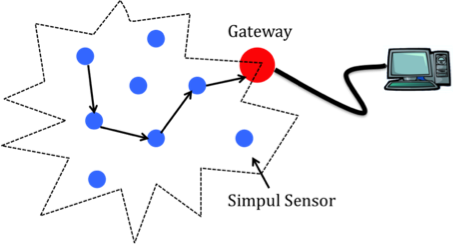
\includegraphics{images/wsn}
          \caption{Jaringan sensor nirkabel.}
          \label{wsn}
      \end{figure}


  \subsection{Sublime Text}
    Et affert civibus has. Has ne facer accumsan argumentum, apeirian hendrerit persequeris pro ex. Suscipit vivendum sensibus mea at, vim ei hinc numquam, at dicit timeam dissentiet mel. At patrioque intellegebat sea, error argumentum dissentias sea in.

    Quo no atqui omnesque intellegat, ne nominavi argumentum quo. Eum ei purto oporteat dissentiet, soleat utamur an sit. Et assum dicam interpretaris quo. Cetero alterum ea vel, no possit alterum utroque nec. His fuisset quaestio ad. Has eu tritani incorrupte consequuntur, esse aliquip nec ne.

% Baris ini digunakan untuk membantu dalam melakukan sitasi
% Karena diapit dengan comment, maka baris ini akan diabaikan
% oleh compiler LaTeX.
\begin{comment}
\bibliography{daftar-pustaka}
\end{comment}


%!TEX root = ../skripsi.tex
%-------------------------------------------------------------------------------
%                            BAB III
%               		METODOLOGI PENELITIAN
%-------------------------------------------------------------------------------
\begin{spacing}{2}
\chapter{METODOLOGI PENGEMBANGAN SISTEM}

\section{Metode Pengumpulan Data}
	Penelitian ini dibuat untuk menganalisis konsep implementasi aplikasi berita berbasis \emph{mobile}, sehingga aplikasi dapat berjalan dengan efektif dan efisien. Sebelum penelitian ini dilakukan riset terlebih dahulu untuk menjaring data serta informasi terkait. Tahap pengumpulan data pada penelitian ini dilakukan dengan metode observasi.

	\subsection{Observasi}
		Kegiatan pengumpulan data secara observasi dilakukan dengan mencoba langsung produk sejenis. Selain itu peneliti juga mengamati fitur dan tata letak dari produk sejenis. Kegiatan observasi dilakukan untuk mengetahui fitur dan keunggulan dari aplikasi sejenis lainnya. Kegiatan observasi dilakukan pada aplikasi \emph{mobile} milik NYTimes, Kompas, dan Detikcom.

\section{Kebutuhan Pengembangan Sistem}
	Pengembangan aplikasi berbasis \emph{mobile} membutuhkan perangkat lunak menulis kode aplikasi dan perangkat keras untuk menjalankannya.

	\subsection{Perangkat Keras}
		Spesifikasi perangkat keras yang dibutuhkan untuk mengembangkan aplikasi adalah sebagai berikut:

		\vspace{-0.5cm}

		\begin{enumerate}[a.]
		\itemsep0em
			\item Macbook Air 13"
			\item Memory 4 GB
			\item Harddisk 256 GB
			\item HP Android
			\item iPhone 6
		\end{enumerate}

	\subsection{Perangkat Lunak}
		Perangkat lunak yang dibutuhkan untuk mengembangkan aplikasi adalah sebagai berikut:

		\vspace{-0.5cm}

		\begin{enumerate}[a.]
		\itemsep0em
			\item Sublime Text 3
			\item NodeJS
			\item Reactroton
			\item Web Browser
			\item Git dan Akun Github.com
			\item Akun Travis-CI.com
		\end{enumerate}

\section{Jadwal Penelitian}
	\begin{table}[H]
  \centering
  \caption{Jadwal Penelitian}
  \label{my-label}
  \begin{tabular}{|c|l|l|l|l|}
  \hline
                                & \multicolumn{1}{c|}{}                                    & \multicolumn{3}{c|}{\textbf{Bulan}}                                            \\ \cline{3-5} 
  \multirow{-2}{*}{\textbf{No}} & \multicolumn{1}{c|}{\multirow{-2}{*}{\textbf{Kegiatan}}} & September                & Oktober                  & November                 \\ \hline
  1                             & Pengajuan Judul                                          & \cellcolor[HTML]{656565} &                          &                          \\ \hline
  2                             & Seminar Proposal                                         &                          & \cellcolor[HTML]{656565} &                          \\ \hline
  3                             & Analisis                                                 &                          & \cellcolor[HTML]{656565} &                          \\ \hline
  4                             & Penyelesaian dan Bimbingan                               &                          & \cellcolor[HTML]{656565} &                          \\ \hline
  5                             & Sidang Skripsi                                           &                          &                          & \cellcolor[HTML]{656565} \\ \hline
  \end{tabular}
  \end{table}
\end{spacing}
% Baris ini digunakan untuk membantu dalam melakukan sitasi
% Karena diapit dengan comment, maka baris ini akan diabaikan
% oleh compiler LaTeX.
\begin{comment}
\bibliography{daftar-pustaka}
\end{comment}


%!TEX root = ./template-skripsi.tex
%-------------------------------------------------------------------------------
%                            BAB IV
%               		ANALISIS DAN PERANCANGAN SISTEM
%-------------------------------------------------------------------------------

\chapter{ANALISIS DAN PERANCANGAN SISTEM}
	\section{Analisis Kebutuhan Sistem}
		Habeo perfecto in sea. Ea deleniti gloriatur pri, paulo mediocrem incorrupte sea ei. Ad mollis scripta per. Incorrupte sadipscing ne mel. Mel ex nonumy malorum epicurei.

		Ne per tota mollis suscipit. Ullum labitur vim ut, ea dicit eleifend dissentias sit. Duis praesent expetenda ne sed. Sit et labitur albucius elaboraret. Ceteros efficiantur mei ad. Hendrerit vulputate democritum est at, quem veniam ne has, mea te malis ignota volumus.

		Eros reprimique vim no. Alii legendos volutpat in sed, sit enim nemore labores no. No odio decore causae has. Vim te falli libris neglegentur, eam in tempor delectus dignissim, nam hinc dictas an.
	
	\section{Perancangan Sistem}		
		Habeo perfecto in sea. Ea deleniti gloriatur pri, paulo mediocrem incorrupte sea ei. Ad mollis scripta per. Incorrupte sadipscing ne mel. Mel ex nonumy malorum epicurei.

		\subsection{Diagram Konteks}
			Consul graeco signiferumque qui id, usu eu summo dicunt voluptatum, nec ne simul perpetua posidonium. Eos ea saepe prodesset signiferumque. No dolore possit est. Mei no justo intellegebat definitiones, vis ferri lorem eripuit ad. Solum tritani scribentur duo ei, his an adipisci intellegat.

		\subsection{User Stories}

	\section{Perancangan Antarmuka Sistem}
		Consul graeco signiferumque qui id, usu eu summo dicunt voluptatum, nec ne simul perpetua posidonium. Eos ea saepe prodesset signiferumque. No dolore possit est. Mei no justo intellegebat definitiones, vis ferri lorem eripuit ad. Solum tritani scribentur duo ei, his an adipisci intellegat.

	\section{Perancangan Peluncuran}
			
			
% Baris ini digunakan untuk membantu dalam melakukan sitasi.
% Karena diapit dengan comment, maka baris ini akan diabaikan
% oleh compiler LaTeX.
\begin{comment}
\bibliography{daftar-pustaka}
\end{comment}

%!TEX root = ./template-skripsi.tex
%-------------------------------------------------------------------------------
%                            	BAB V
%               		KESIMPULAN DAN SARAN
%-------------------------------------------------------------------------------

\chapter{KESIMPULAN DAN SARAN}

\section{Kesimpulan}
	Berdasarkan hasil analisis dan pengujian fungsional aplikasi ini, didapat kesimpulan sebagai berikut:

	\begin{enumerate}
		\item Lorem ipsum is a pseudo-Latin text used in web design, typography, layout, and printing in place of English to emphasise design elements over content. 
		
		\item It's also called placeholder (or filler) text. It's a convenient tool for mock-ups. 
		
		\item It helps to outline the visual elements of a document or presentation, eg typography, font, or layout. Lorem ipsum is mostly a part of a Latin text by the classical author and philospher Cicero.

		\item Its words and letters have been changed by addition or removal, so to deliberately render its content nonsensical; it's not genuine, correct, or comprehensible Latin anymore. 
	\end{enumerate}


\section{Saran}
	\begin{enumerate}
		\item Lorem ipsum is a pseudo-Latin text used in web design, typography, layout, and printing in place of English to emphasise design elements over content. 
		
		\item It's also called placeholder (or filler) text. It's a convenient tool for mock-ups. 
		
		\item It helps to outline the visual elements of a document or presentation, eg typography, font, or layout. Lorem ipsum is mostly a part of a Latin text by the classical author and philospher Cicero.

		\item Its words and letters have been changed by addition or removal, so to deliberately render its content nonsensical; it's not genuine, correct, or comprehensible Latin anymore. 
	\end{enumerate}

	
% Baris ini digunakan untuk membantu dalam melakukan sitasi
% Karena diapit dengan comment, maka baris ini akan diabaikan
% oleh compiler LaTeX.
\begin{comment}
\bibliography{daftar-pustaka}
\end{comment}


%-----------------------------------------------------------------
%Disini akhir masukan Bab
%-----------------------------------------------------------------


%-----------------------------------------------------------------
% Disini awal masukan untuk Daftar Pustaka
% - Daftar pustaka diambil dari file .bib yang ada pada folder ini
%   juga.
% - Untuk memudahkan dalam memanajemen dan menggenerate file .bib
%   gunakan reference manager seperti Mendeley, Zotero, EndNote,
%   dll.
%-----------------------------------------------------------------
\bibliography{IEEEabrv,daftar-pustaka}
\addcontentsline{toc}{chapter}{DAFTAR PUSTAKA}
%-----------------------------------------------------------------
%Disini akhir masukan Daftar Pustaka
%-----------------------------------------------------------------

\end{document}